
%(BEGIN_QUESTION)
% Copyright 2007, Tony R. Kuphaldt, released under the Creative Commons Attribution License (v 1.0)
% This means you may do almost anything with this work of mine, so long as you give me proper credit

Qualitatively graph the individual proportional, integral, and derivative responses of a PID controller to the following input conditions, assuming {\it direct} controller action.  Use a solid line for proportional, a dashed line for integral, and a dotted line for derivative:

$$\includegraphics[width=15.5cm]{i01638x01.eps}$$

Then, draw a final graph of the controller's output, showing how the P, I, and D terms would combine to form a composite waveform:

$$\includegraphics[width=15.5cm]{i01638x01.eps}$$

\vskip 20pt \vbox{\hrule \hbox{\strut \vrule{} {\bf Suggestions for Socratic discussion} \vrule} \hrule}

\begin{itemize}
\item{} Many students find the task of summing all three control actions together to be much more difficult than plotting any of the three responses separately.  Devise a problem-solving strategy to ensure your summation will always be correct!
\end{itemize}

\underbar{file i01638}
%(END_QUESTION)





%(BEGIN_ANSWER)

The controller output graph shown here is {\it qualitative} only.  Although drawn to scale (i.e. all changes in the output are properly scaled relative to each other), the scale itself is arbitrary and therefore may not match the scale of your sketch:

\vskip 10pt

Individual P, I, and D responses graphed:

$$\includegraphics[width=15.5cm]{i01638x02.eps}$$

Final output signal graph:

$$\includegraphics[width=15.5cm]{i01638x03.eps}$$

%(END_ANSWER)





%(BEGIN_NOTES)



%INDEX% Control, proportional + integral + derivative: graphing controller response

%(END_NOTES)


